\section{Description séquentielle des modules}
    \label{sec:modules}
    
Le diagramme de séquence présenté dans cette section a pour objectif d'illustrer le fonctionnement des trois principales fonctionnalités de Glasir : le Filtre, l'Optimiseur et l'Editeur de fonction. Pour mieux saisir le fonctionnement de l'un de ces modules, la {\sc Figure}~{\ref{fig:start}} illustre l'ouverture d'un ADTree dans Glasir.

Pour rappel, la lecture d'un diagramme de séquence se fait de haut en bas, suivant un ordre chronologique, et en suivant les flèches, qui correpondent aux méthodes des différentes classes présentées en tête du diagramme. On peut donc suivre de cette manière l'ordre d'activité des différentes classes au cours d'une utilisation donnée, ici celle d'un module de Glasir (le Filtre, l'Éditeur de fonctions ou l'Optimiseur).

Ainsi, sur la {\sc Figure}~{\ref{fig:start}}, l'expert en sécurité demande à ouvrir un fichier XML contenant un ADTree dans Glasir. Ce dernier crée alors une instance d'ADTool, qui va chercher le code XML du fichier afin d'afficher l'ADTree.

	    \begin{figure}[H]
	        \centering
	        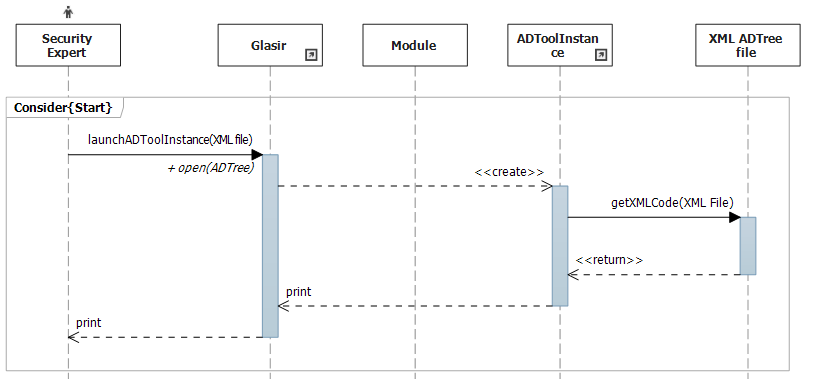
\includegraphics[height=0.5\textwidth]{figure/startseqdiag.png}
	        \caption{Diagramme de séquence du démarrage d'une instance d'ADTool dans Glasir.}
	        \label{fig:start}
	    \end{figure}
	    
	    La {\sc Figure}~{\ref{fig:moduleseq}} illustre le fonctionnement générique d'un module. L'expert en sécurité spécifie d'abord les paramètres de l'opération que va effectuer le module. Puis, une fois lancé, le module va effectuer des opérations sur le fichier de l'ADTree cible. Un fichier résultat est alors généré puis ouvert dans une nouvelle instance d'ADTool, afin d'être affiché à l'écran. 

	    \begin{figure}[H]
	        \centering
	        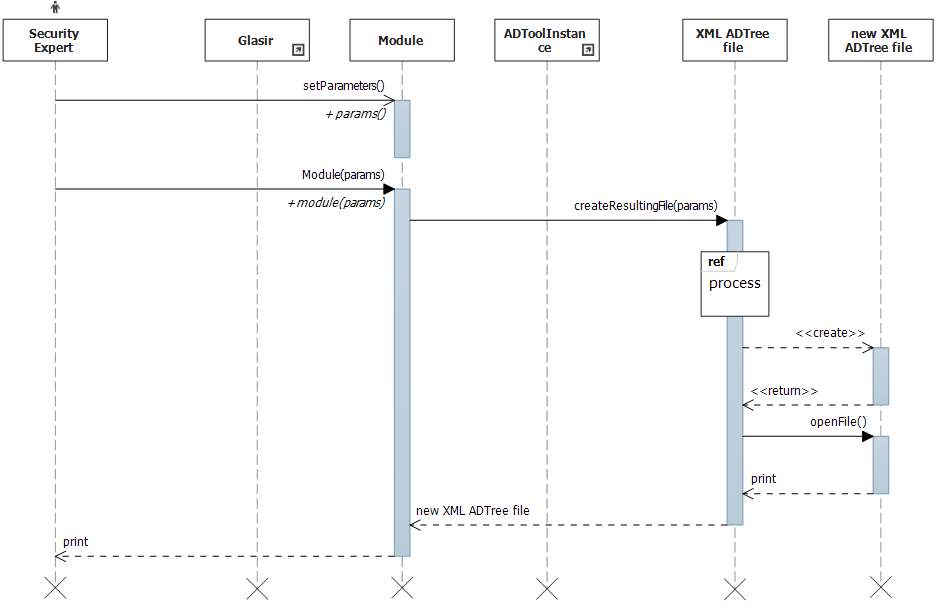
\includegraphics[height=0.75\textwidth]{figure/moduleSeqDiag.png}
	        \caption{Diagramme de séquence générique d'un module, qui ne correspond d'ailleurs pas exactement à la description. Il faut légèrement le modifier.}
	        \label{fig:moduleseq}
	    \end{figure}

Par exemple, dans le cas du Filtre, les paramètres du module sont les intervalles\footnote{ADTool propose des paramètres de valuation tels que le coût d'une attaque (un nombre réel) ou sa faisabilité (un booléen). Bien que certains de ces paramètres soient définis sur un ensemble discret, il est toujours possible de définir une relation d'ordre sur cet ensemble, et donc d'y définir des intervalles.} de filtrage sur les valuations de l'ADTree. Pour l'Editeur de fonctions, le paramètre est la définition de la fonction. Enfin, pour l'Optimiseur, il s'agit du paramètre d'ADTool selon lequel l'expert souhaite optimiser l'ADTree.